\chapter{Further Plots and Tables}
\label{ap:more_plots}

\section{t-SNE plots for the data from \cite{Derrac2015}}

\begin{figure}[h]
	\begin{center}
	  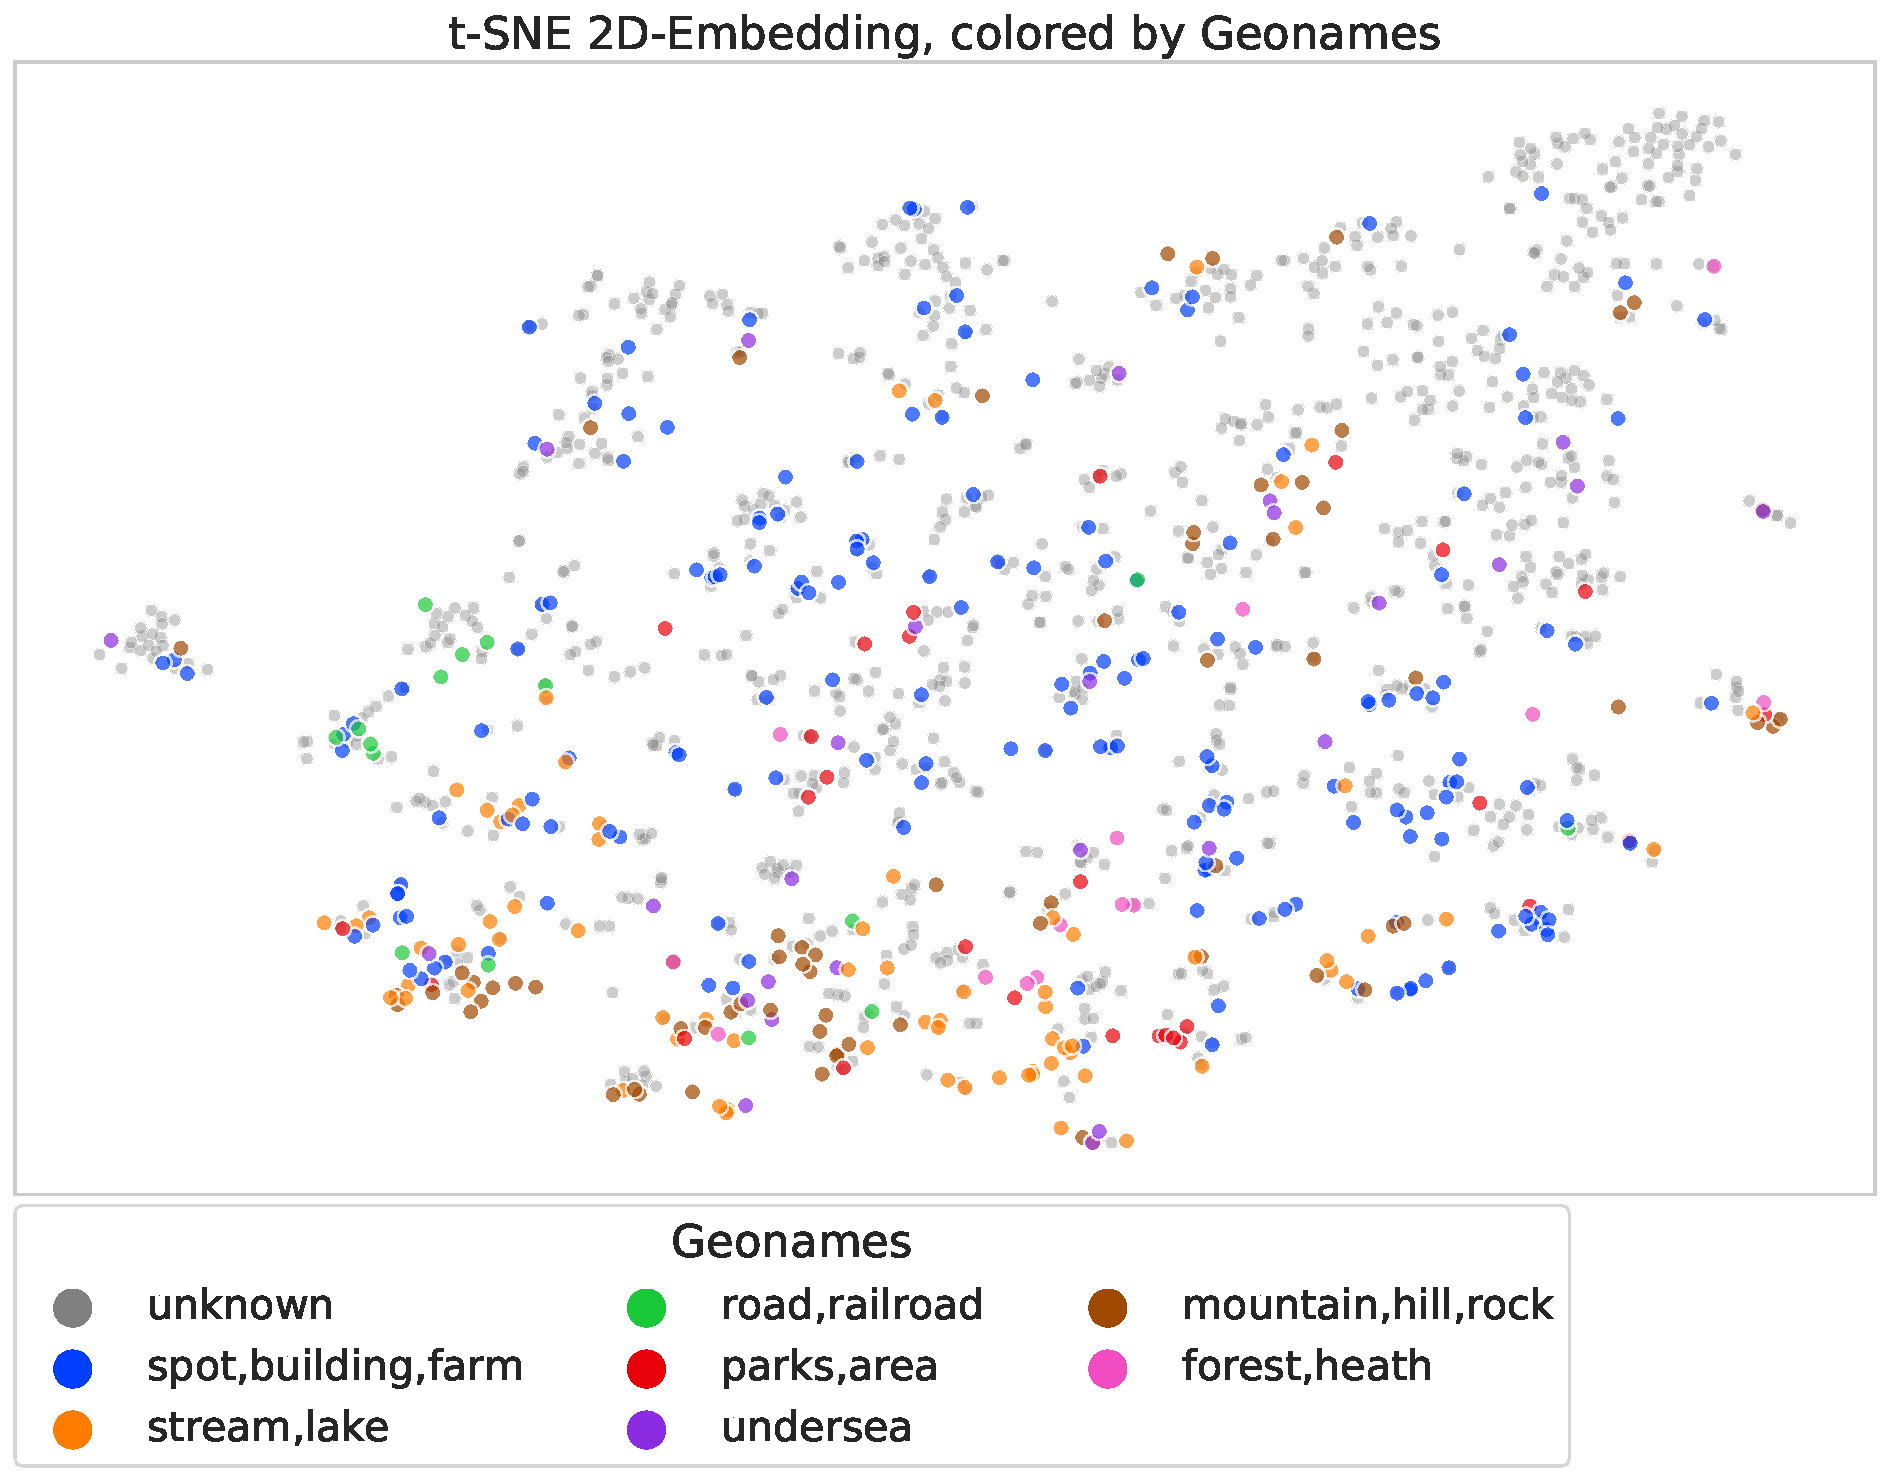
\includegraphics[width=\textwidth]{graphics/figures/scatter_mds_tsne_places_Geonames.pdf}
	  \caption[2D visualization of the placetypes-dissimilarity matrix]{2D visualization of the placetypes-dissimilarity matrix for the data uploaded by \textcite{Derrac2015}, colored by GeoNames. Generated with \gls{tsne}. See \url{https://github.com/cstenkamp/derive_conceptualspaces/blob/main/notebooks/text_referenced_plots/desc15_mds_2d3d.ipynb} for the origin of this plot. Individual class frequencies: spot,building,farm: 176 | stream,lake: 74 | mountain,hill,rock: 68 | parks,area: 28 | undersea: 27 | road,railroad: 16 | forest,heath: 14}
	  \label{fig:scatter_mds_placetypes}
      %TODO: "colored by GeoNames"
	\end{center}
\end{figure}

F
\begin{figure}[h]
	\begin{center}
	  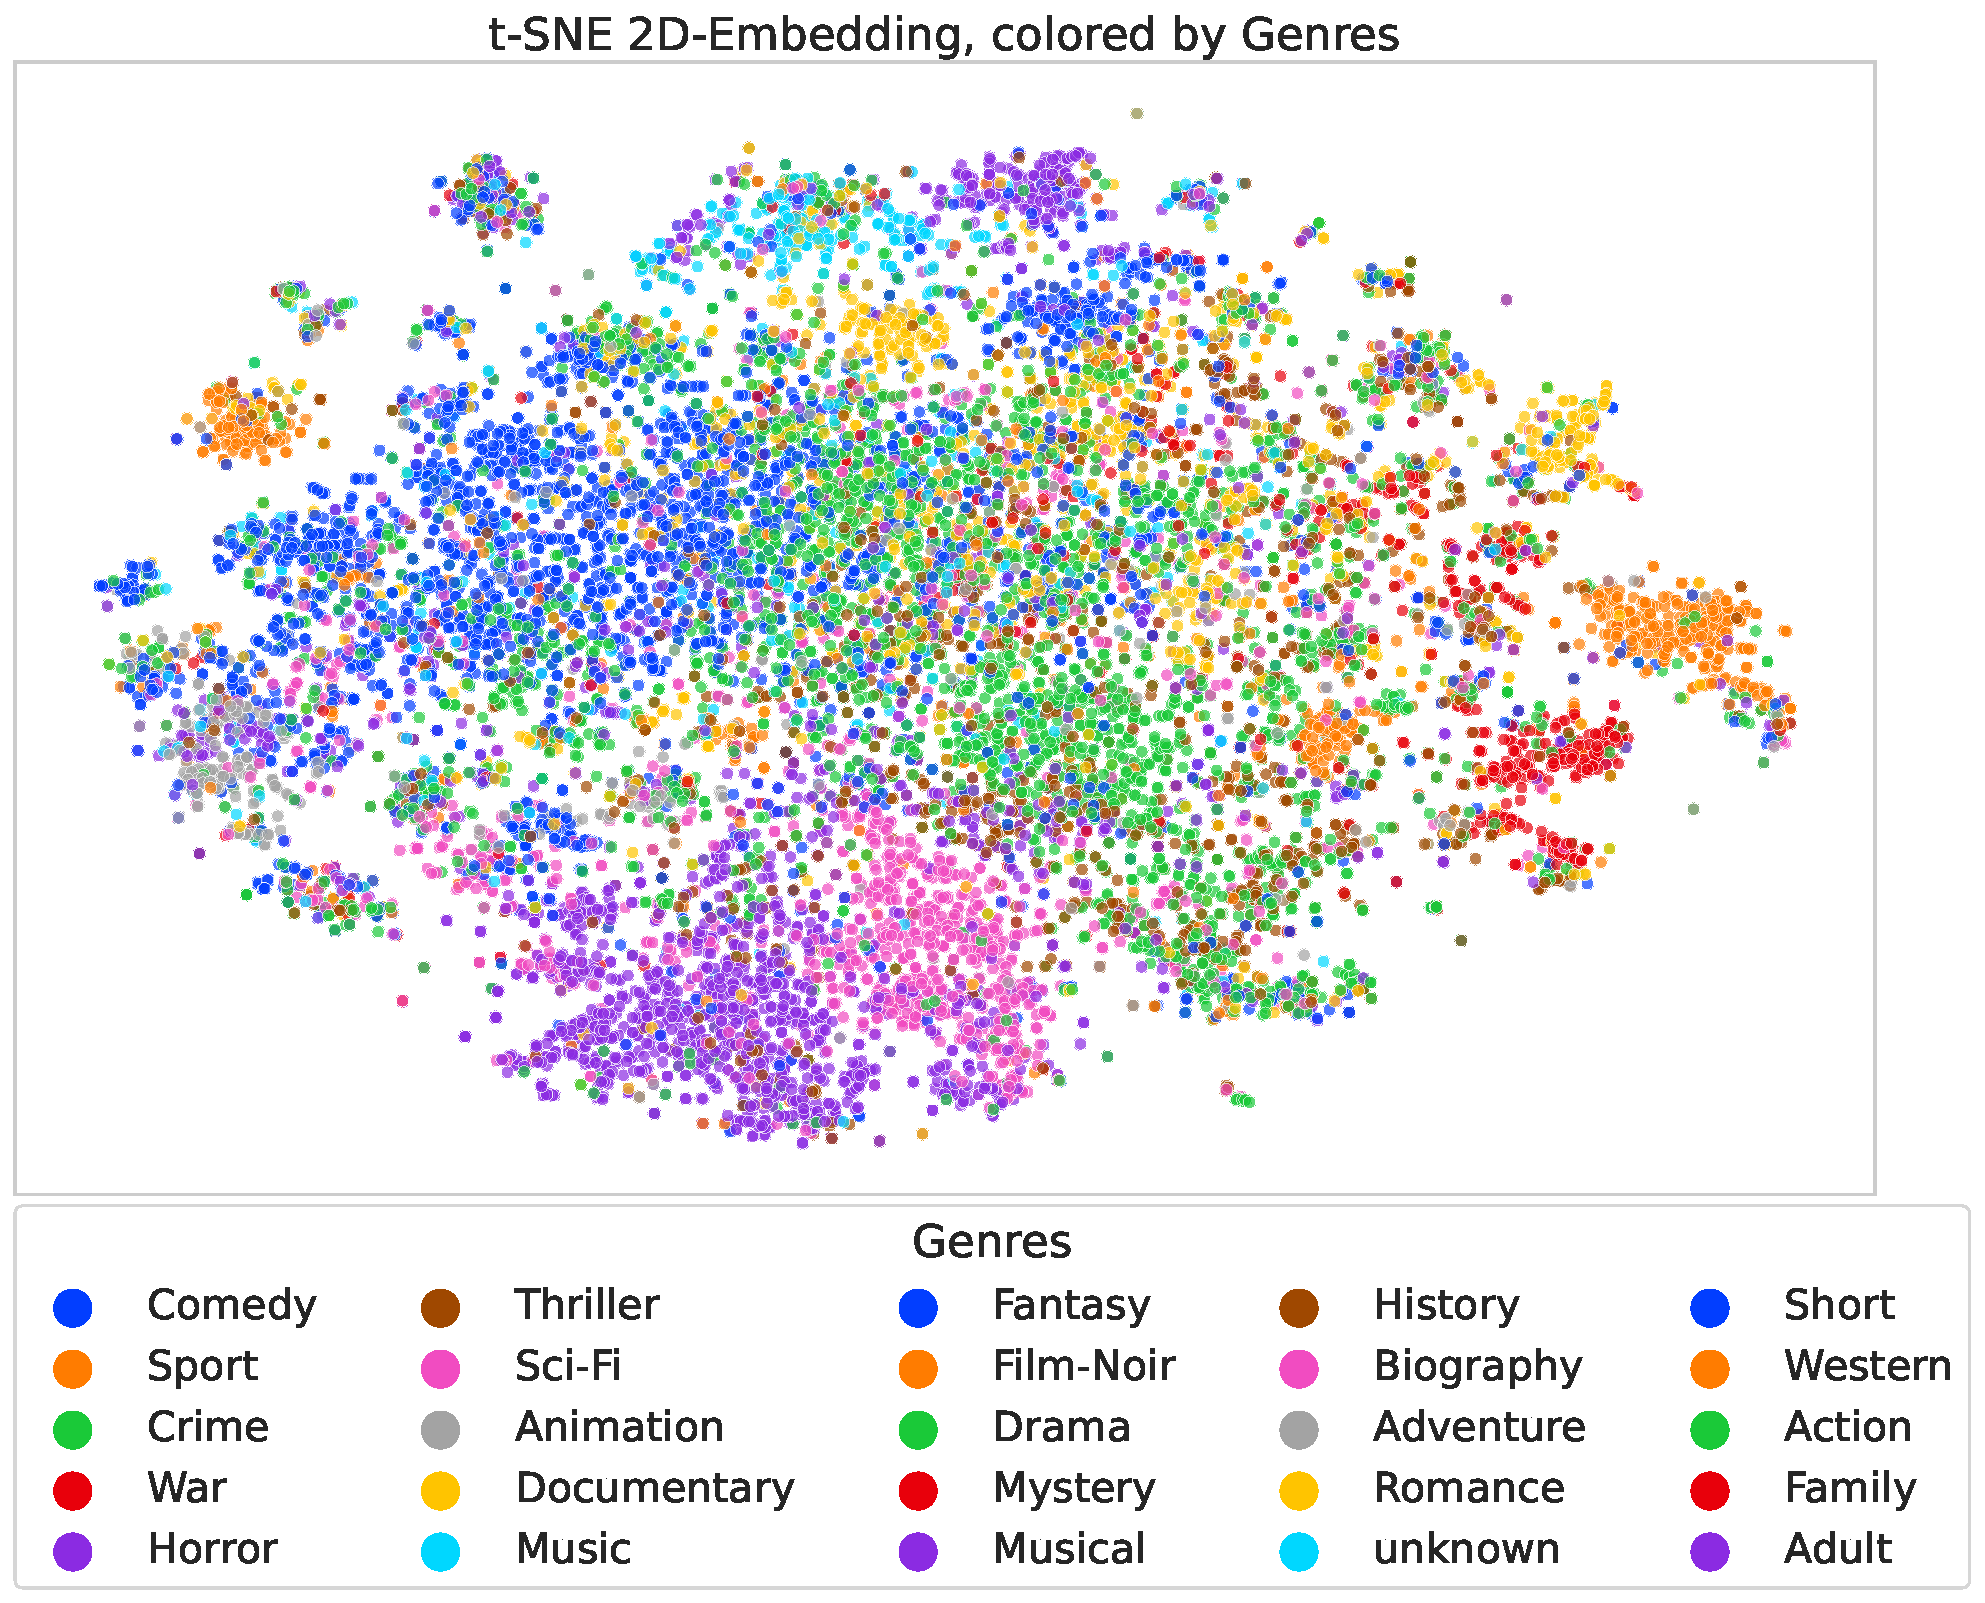
\includegraphics[width=\textwidth]{graphics/figures/scatter_mds_tsne_movies_Genres.pdf}
	  \caption[2D visualization of the movies-dissimilarity matrix]{2D visualization of the movies-dissimilarity matrix for the data uploaded by \textcite{Derrac2015}, colored by genre. Generated with \gls{tsne}. See \url{https://github.com/cstenkamp/MAAnalysisNotebooks/blob/main/analyze_results/derrarc2015/mds_derrac2015_moviesplaces_2d3d.ipynb} for the origin of this plot.}
	  \label{fig:scatter_mds_movies}
	\end{center}
\end{figure}

% \todo
Note that at \url{https://github.com/cstenkamp/MAAnalysisNotebooks/blob/main/analyze_results/derrarc2015/mds_derrac2015_moviesplaces_2d3d.ipynb} there are also interactive 3D-Versions of these plots. The one for the Siddata-dataset is at \url{https://github.com/cstenkamp/derive_conceptualspaces/blob/main/notebooks/text_referenced_plots/visualise_embeddings.ipynb}, also 2D and interactive 3D. 

\clearpage
\section{Results for Classifiers on placetypes}

\begin{table}[H]
	\centering
	\makebox[\textwidth][c]{
		\resizebox{1.16\textwidth}{!}{%
		\begin{tabular}{r@{}r|ccccc|ccccc|cc|ccc}
		&
		&
		\multicolumn{5}{c|}{\textbf{\textcite{Alshaikh2020} (MDS)}} &
		\multicolumn{5}{c|}{\textbf{\textcite{Ager2018}}} &
		\multicolumn{2}{c|}{\textbf{{\scriptsize Der. \& Sch.} \cite{Derrac2015}}} &
		\multicolumn{3}{c}{\textbf{This work}} \\
		&
		&
		\textbf{\footnotesize Rand.} &
		\textbf{AHC} &
		\textbf{\footnotesize Prim.} &
		\textbf{Sub} &
		\textbf{\footnotesize Ortho} &
		\textbf{\footnotesize FTMDS} &
		\textbf{MDS} &
		\textbf{\footnotesize FTAWV} &
		\textbf{AWV} &
		\textbf{LDA} &
		\textbf{Best} &
		\textbf{\footnotesize Best BL} &
		\textbf{B-all} &
		\textbf{Avg-B} &
		\textbf{A-UnW} \\ \midrule
		\multirow[t]{2}{*}{\specialcell[t]{\textbf{Four-}\\ \textbf{square}}} &
		\textbf{D1} &
		0.39 &
		0.36 &
		0.36 &
		0.43 &
		\textbf{0.45} &
		0.41 &
		0.38 &
		0.39 &
		0.32 &
		\textbf{0.55} &
		\multicolumn{2}{c|}{-} &
		\textbf{0.50} & 0.45 & 0.36
		\\
		&
		\textbf{D3} &
		0.50 &
		0.46 &
		0.48 &
		0.54 &
		\textbf{0.57} &
		0.44 &
		0.42 &
		0.42 &
		0.37 &
		0.48 &
		\multicolumn{2}{c|}{-} &
		\textbf{0.58} & 0.5 & 0.54
		\\
		&
		\textbf{DN} &
		\multicolumn{5}{c|}{-} &
		0.41 &
		0.42 &
		0.41 &
		0.31 &
		0.47 &
		\textbf{0.53} &
		\textbf{0.53} &
		\textbf{0.57} & 0.55 & 0.54
		\\
		\multicolumn{1}{l}{} &
		\multicolumn{1}{l|}{\textbf{Any}} &
		\multicolumn{5}{c|}{-} &
		\multicolumn{5}{c|}{-} &
		\textbf{0.73} &
		0.72 &
		- & - & -
		\\
		\multirow[t]{2}{*}{\specialcell[t]{\textbf{Geo-}\\ \textbf{names}}} &
		\textbf{D1} &
		0.23 &
		0.22 &
		0.24 &
		0.20 &
		0.28 &
		0.32 &
		\textbf{0.32} &
		0.31 &
		0.28 &
		\textbf{0.34} &
		\multicolumn{2}{c|}{-} &
		\textbf{0.51} & 0.48 & 0.49
		\\
		&
		\textbf{D3} &
		0.27 &
		0.29 &
		0.27 &
		0.32 &
		\textbf{0.34} &
		0.31 &
		0.31 &
		0.29 &
		0.28 &
		0.32 &
		\multicolumn{2}{c|}{-} &
		\textbf{0.54} & 0.51 & 0.29
		\\
		&
		\textbf{DN} &
		\multicolumn{5}{c|}{-} &
		0.24 &
		0.21 &
		0.23 &
		0.22 &
		0.27 &
		\textbf{0.37} &
		0.2 &
		\textbf{0.46} & 0.44 & 0.42
		\\
		\multicolumn{1}{l}{} &
		\multicolumn{1}{l|}{\textbf{Any}} &
		\multicolumn{5}{c|}{-} &
		\multicolumn{5}{c|}{-} &
		\textbf{0.41} &
		0.36 &
		- & - & -
		
		\end{tabular}%
		} % resizebox
	} % makebox
	\caption[F1-scores of classifiers for placetype-taxonomies of \mainalgos and this work (long)]{F1-scores of classifiers predicting GeoNames- and Foursquare-labels for three baselines, \mainalgos and this work. (long). Described in detail below.}
	\label{tab:f1_placetypes_long}
\end{table}


\autoref{tab:f1_placetypes_long} is a longer version of \autoref{tab:f1_mainalgos_me_short}, reporting F1-Scores of classifiers predicting GeoNames- and Foursquare-labels for baselines, \mainalgos and this work. 
\textbf{Cls} column encodes the classifier: \textbf{D1/3} are \glspl{dt} of depth 1/3, \textbf{DN} an unbounded \gls{dt}. Condition \textbf{Any} refers to the best of all semantic classifiers developed by \cite{Derrac2015}. \\
First five columns are the exact results reported by \cite{Alshaikh2020}, next five columns those by \cite{Ager2018}, afterwards the best config of \cite{Derrac2015} and the best baseline-condition of \cite{Derrac2015}. The exact conditions of that work are (left to right, top to bottom): C4.5\textsubscript{dir}, C4.5\textsubscript{MDS}, Col, 1-NN (100D), C4.5\textsubscript{dir}, C4.5\textsubscript{MDS}, Analog\textsubscript{C}, 1-NN (50D). Explanations of the respective conditions can be found in their work. \\
All scores are reported with a train-test split of 70\% to 30\%. Note that the reported results of \cite{Ager2018} are unrepresentive when compared to the other datasets: For the placetypes-dataset, \textbf{LDA} performs consistently better than their methods, which is not the case for all other datasets used by them. In the case of \cite{Alshaikh2020}, the results for the placetypes-dataset seem to indicate that the \textbf{Ortho}-condition performs consistently better than the \textbf{Sub}-condition, which was however not the case for any of the other datasets the authors considered. \\
Final columns are the results of this work. Column \textbf{Best-all} encodes a different for each row, specifically the one that yields the best result for the respective classification task, whereas column \textbf{Mean-Best} refers to the single configuration that achieved the best results on average. Last column is best when class weighting of per-class-classifiers is forbidden.
\todoparagraph{Shortened a few column names, rename them in description}

\section{Comparison of different Cluster-Center-Algorithms}

\todoparagraph{We compared reclassify and main on placetypes. For both of the techniques, we show the entitiy that scored highest}

\begin{table}[H]
	\centering
	\begin{tabular}{r|ll}
	\textbf{Dimension}               & \textbf{reclassify} & \textbf{main}       \\ \midrule
	\textbf{isawyoufirst}            & beach               & beach               \\
	\textbf{workspace}               & office              &                     \\
	\textbf{nutrition}               & restaurant          & deli                \\
	\textbf{goalie}                  & stadium             & footballstadium     \\
	\textbf{pumperbuilding}          & county              &                     \\
	\textbf{starwoodhotels}          & hotelroom           & pool                \\
	\textbf{interstate10}            & highway             & mongolianrestaurant \\
	\textbf{urban}                   & interior            & movietheater        \\
	\textbf{tuolumne}                & creek               & nationalforest      \\
	\textbf{cabs}                    & downtown            &                     \\
	\textbf{investment}              & school              & stockexchange       \\
	\textbf{stripmall}               & downtown            & departmentstore     \\
	\textbf{michiganstateuniversity} & school              & campus              \\
	\textbf{ews}                     & railroad            & train               \\
	\textbf{anchored}                & boat                & pier                \\
	\textbf{a10}                     & airport             &                     \\
	\textbf{wc2}                     & restaurant          & square              \\
	\textbf{airbase}                 & airport             & airbase             \\
	\textbf{joshuatreenationalpark}  & canyon              &                     \\
	\textbf{clinker}                 & building            &                    
	\end{tabular}
	\caption[Highest-ranking descriptions per dimension for different algorithms]{Highest-ranking descriptions per dimension for the reclassify-algorithm and the main-algorithm}
	\label{tab:text_per_dim}
\end{table}

% We see that using the respectively best-fitting DOCUMENT (without LSI or anything, just the one with the highest ranking!)  is often even the MUCH BETTER direction!!! 



\section{F1-scores per faculty}


\begin{table}[H]
	\resizebox{\textwidth}{!}{%
		\begin{tabular}{rcccc}
		\toprule
		\textbf{Depth} & \textbf{1} & \textbf{2} & \textbf{3} & \textbf{unbound} \\
		\midrule
		\textbf{Sozialwissenschaften} & 0.386 ± 0.029 & 0.414 ± 0.031 & 0.403 ± 0.024 & 0.580 ± 0.034 \\
		\textbf{Kultur-/Geowissenschaften} & 0.454 ± 0.023 & 0.514 ± 0.034 & 0.591 ± 0.026 & 0.685 ± 0.020 \\
		\textbf{Erziehungs-/Kulturwissenschaften} & 0.600 ± 0.019 & 0.701 ± 0.015 & 0.713 ± 0.019 & 0.765 ± 0.015 \\
		\textbf{Physik} & 0.096 ± 0.019 & 0.117 ± 0.012 & 0.145 ± 0.023 & 0.552 ± 0.072 \\
		\textbf{Biologie/Chemie} & 0.133 ± 0.019 & 0.178 ± 0.043 & 0.247 ± 0.063 & 0.611 ± 0.084 \\
		\textbf{Mathematik/Informatik} & 0.215 ± 0.032 & 0.211 ± 0.046 & 0.260 ± 0.057 & 0.542 ± 0.070 \\
		\textbf{Sprach-/Literaturwissenschaften} & 0.652 ± 0.020 & 0.685 ± 0.014 & 0.733 ± 0.014 & 0.790 ± 0.017 \\
		\textbf{Humanwissenschaften} & 0.177 ± 0.028 & 0.245 ± 0.061 & 0.276 ± 0.078 & 0.484 ± 0.043 \\
		\textbf{Wirtschaftswissenschaften} & 0.198 ± 0.022 & 0.219 ± 0.059 & 0.236 ± 0.040 & 0.596 ± 0.084 \\
		\textbf{Rechtswissenschaften} & 0.617 ± 0.108 & 0.456 ± 0.037 & 0.641 ± 0.050 & 0.841 ± 0.032 \\
		\textbf{Mean (weighted)} & 0.505 ± 0.026 & 0.553 ± 0.026 & 0.597 ± 0.026 & 0.710 ± 0.026 \\
		\textbf{Mean (unweighted)} & 0.353 ± 0.032 & 0.374 ± 0.035 & 0.424 ± 0.039 & 0.645 ± 0.047 \\
		\bottomrule
		\end{tabular}
	}
	\slcaption{Robust F1-scores per faculty of a well-performing configuration. The reported results are mean and standard deviation from the result of ten runs with 5-fold crossvalidation each. \backref{tab:robustresults_perfb}}
	\label{tab:robustresults_perfb_f1}
\end{table}


\section{Sample Classification}


\begin{figure}[h]
	\begin{center}
	  \makebox[\textwidth][c]{
		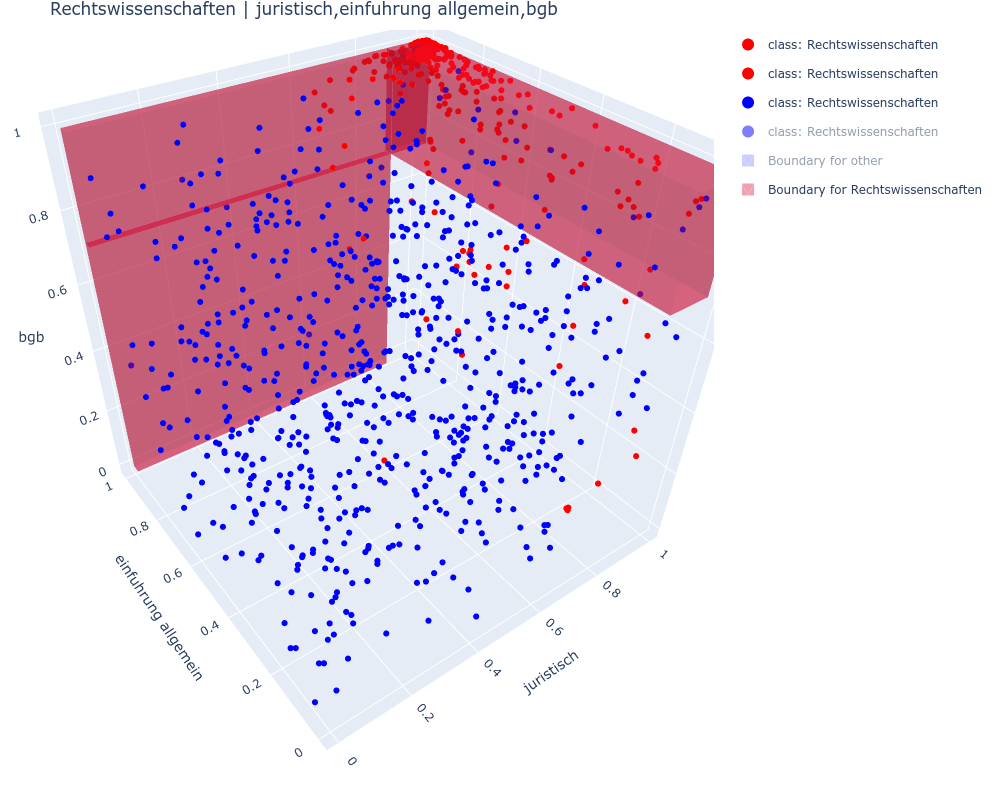
\includegraphics[width=1.1\textwidth]{graphics/dataset_new/boxes_rechtswis.png}
		\slcaption{Sample classification of a level-2-decisiontree. visualise in 3D: \url{https://github.com/cstenkamp/derive_conceptualspaces/blob/main/notebooks/text_referenced_plots/display_top3_SIDDATA.ipynb} \arrowback}
		\label{fig:boxes_rechtswis}
		% möchte sagen: How does a decision look graphically, and how does it compare to the original 3D?
		% TODO: add accuracy 
	  }
	\end{center}
\end{figure}


\section{Box-plots}

\begin{figure}[h]
	\begin{center}
	  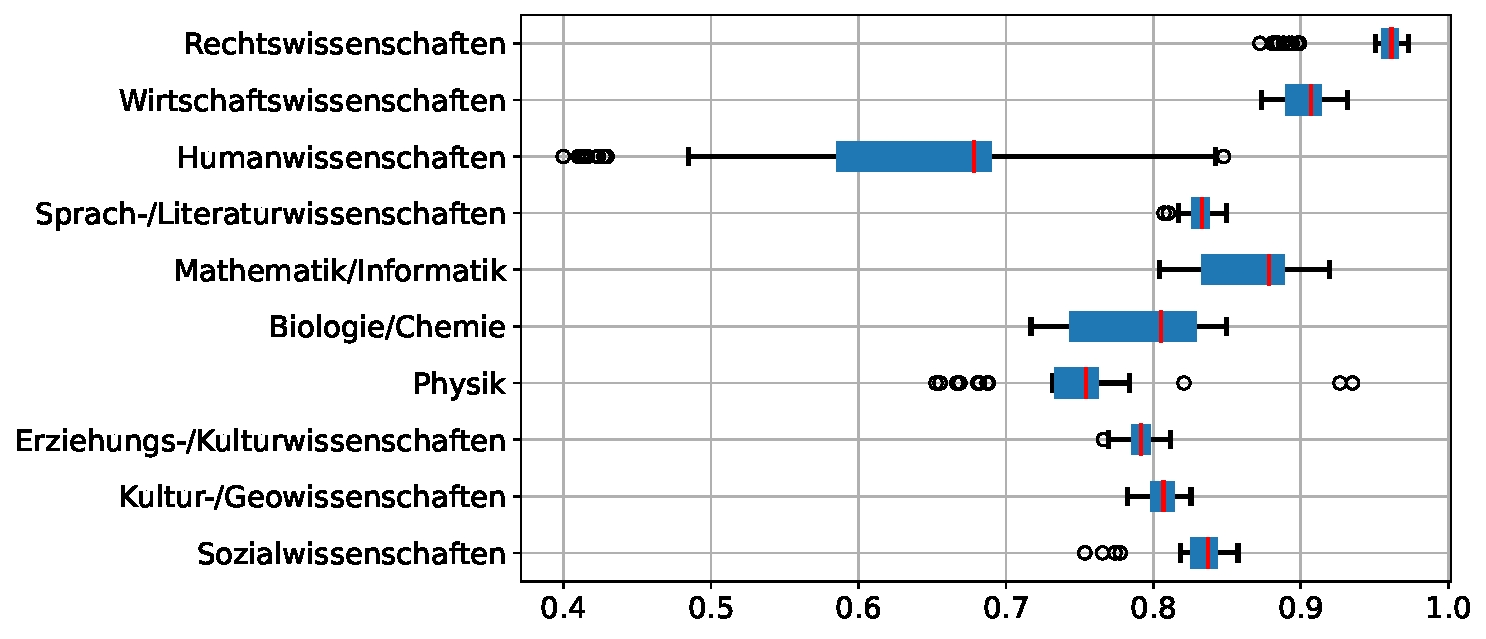
\includegraphics[width=\textwidth]{graphics/dataset_new/accuracy_boxplots.pdf}
	  \slcaption{Variability of faculty classification cccuracy as box-plots.}
	  \label{fig:faculty_boxplots}
	\end{center}
\end{figure}


\section{Dataset samples}

\begin{table}[H]
	\centering
	\resizebox{\textwidth}{!}{%
	\begin{tabular}{ll}
	\textbf{Number} & \textbf{Course} \\
	1.003                  & Spez. Soz. III: Wahlforschung (Politische Soziologie)               \\
	1.003                  & Erziehung, Bildung und Sozialisation in der modernen Gesellschaft   \\
	1.003                  & Infoveranstaltung Master Soziologie                                 \\
	7.441202               & "Fremdheit" in der Kinder- und Jugendliteratur                      \\
	7.441202               & „Mündlichkeit und Schriftlichkeit“                         
	\end{tabular}%
D	}
	\caption{Sample duplicates in the Siddata-dataset. }
	\label{tab:sample_duplicates}
\end{table}



% \begin{table}[H]
% 	\centering
% 	\begin{tabular}{lll}
% 	\textbf{Description}  \\
% 		                   & BA/MA Hauptmodul \\
% 		                   & Bestandteile:Vorlesung + Übung \\
% 		                   & Dozent  Dr. Michael Wicke \\
% 			               & Siehe Gruppe A \\
% 			               & „s. Modulbeschreibung \\
% 						   & Literatur:wird noch bekannt gegeben
% 	\end{tabular}%
% 	\caption{Low quality data samples \todoparagraph{(from data_exploration_Siddata2021)}}
% 	\label{tab:sample_descriptions}
% \end{table}


\section{Hyperparameter search}


\begin{table}[h]
	\resizebox{\textwidth}{!}{%
	\begin{tabular}{llllrrrrrrrrr}
	\toprule
% 	 &  &  &  & \rotatebox{70}{\textbf{k_r2r_d}} & \rotatebox{70}{\textbf{k_r2r_min}} & \rotatebox{70}{\textbf{k_dig}} & \rotatebox{70}{\textbf{k_r2r+_d}} & \rotatebox{70}{\textbf{k_r2r+_min}} & \rotatebox{70}{\textbf{k_r2r+_max}} & \rotatebox{70}{\textbf{k_dig+_2}} & \rotatebox{70}{\textbf{k_c2r+}} & \rotatebox{70}{\textbf{mean}} \\
	\textbf{Preprocessing} & \specialcell[b]{\textbf{Quanti-}\\ \textbf{fication}} & \textbf{\#Dims} & \specialcell[b]{\textbf{Doc-Term-}\\ \textbf{Matrix} \\ \textbf{Quanti-}\\ \textbf{fication}} & \rotatebox{70}{\textbf{k_r2r_d}} & \rotatebox{70}{\textbf{k_r2r_min}} & \rotatebox{70}{\textbf{k_dig}} & \rotatebox{70}{\textbf{k_r2r+_d}} & \rotatebox{70}{\textbf{k_r2r+_min}} & \rotatebox{70}{\textbf{k_r2r+_max}} & \rotatebox{70}{\textbf{k_dig+_2}} & \rotatebox{70}{\textbf{k_c2r+}} & \rotatebox{70}{\textbf{mean}} \\
	\midrule
	\multirow[t]{24}{*}{\mfauhcsdT} & \multirow[t]{8}{*}{\textbf{count}} & \multirow[t]{2}{*}{\textbf{3}} & \textbf{ppmi} & 0 & 1 & 0 & 145 & 370 & 510 & 191 & - & 174 \\
	 &  &  & \textbf{tfidf} & 0 & 1 & 0 & 110 & 237 & 278 & 83 & - & 101 \\
	\cline{3-4}
	 &  & \multirow[t]{3}{*}{\textbf{100}} & \textbf{count} & 0 & 5 & 0 & 0 & 114 & 52 & 290 & 0 & 58 \\
	 &  &  & \textbf{ppmi} & 0 & 6 & 27 & 139 & 224 & 247 & 120 & - & 109 \\
	 &  &  & \textbf{tfidf} & 0 & 6 & 5 & 246 & 270 & 281 & 201 & - & 144 \\
	\cline{3-4}
	 &  & \multirow[t]{3}{*}{\textbf{200}} & \textbf{count} & 0 & 5 & 1 & 0 & 133 & 52 & 509 & 0 & 88 \\
	 &  &  & \textbf{ppmi} & 0 & 6 & 57 & 196 & 315 & 344 & 90 & - & 144 \\
	 &  &  & \textbf{tfidf} & 0 & 6 & 17 & 357 & 370 & 372 & 433 & - & 222 \\
	\cline{2-4} \cline{3-4}
	 & \multirow[t]{8}{*}{\textbf{ppmi}} & \multirow[t]{2}{*}{\textbf{3}} & \textbf{ppmi} & 0 & 0 & 0 & 192 & 247 & 363 & 136 & - & 134 \\
	 &  &  & \textbf{tfidf} & 0 & 0 & 0 & 169 & 206 & 217 & 59 & - & 93 \\
	\cline{3-4}
	 &  & \multirow[t]{3}{*}{\textbf{100}} & \textbf{count} & 0 & 0 & 0 & 0 & 38 & 25 & 242 & 0 & 38 \\
	 &  &  & \textbf{ppmi} & 0 & 0 & 0 & 80 & 112 & 101 & 22 & - & 45 \\
	 &  &  & \textbf{tfidf} & 0 & 0 & 0 & 89 & 90 & 96 & 85 & - & 51 \\
	\cline{3-4}
	 &  & \multirow[t]{3}{*}{\textbf{200}} & \textbf{count} & 0 & 0 & 0 & 0 & 34 & 21 & 293 & 0 & 44 \\
	 &  &  & \textbf{ppmi} & 0 & 1 & 112 & 100 & 163 & 163 & 37 & - & 82 \\
	 &  &  & \textbf{tfidf} & 0 & 1 & {\cellcolor{lightgreen}} 127 & 99 & 107 & 106 & 131 & - & 82 \\
	\cline{2-4} \cline{3-4}
	 & \multirow[t]{8}{*}{\textbf{tfidf}} & \multirow[t]{2}{*}{\textbf{3}} & \textbf{ppmi} & 0 & 0 & 0 & 229 & 357 & 423 & 84 & - & 156 \\
	 &  &  & \textbf{tfidf} & 0 & 0 & 0 & 169 & 255 & 258 & 24 & - & 101 \\
	\cline{3-4}
	 &  & \multirow[t]{3}{*}{\textbf{100}} & \textbf{count} & 0 & 1 & 0 & 0 & 162 & 64 & 450 & 0 & 85 \\
	 &  &  & \textbf{ppmi} & 0 & 1 & 3 & 324 & 404 & 423 & 151 & - & 187 \\
	 &  &  & \textbf{tfidf} & 0 & 1 & 0 & 390 & 422 & 437 & 425 & - & 239 \\
	\cline{3-4}
	 &  & \multirow[t]{3}{*}{\textbf{200}} & \textbf{count} & 0 & 2 & 0 & 0 & 211 & 83 & {\cellcolor{lightgreen}} 869 & {\cellcolor{lightgreen}} 1 & 146 \\
	 &  &  & \textbf{ppmi} & 0 & 2 & 13 & 395 & {\cellcolor{lightgreen}} 559 & {\cellcolor{lightgreen}} 577 & 153 & - & 243 \\
	 &  &  & \textbf{tfidf} & 0 & 2 & 0 & {\cellcolor{lightgreen}} 531 & 554 & 572 & 794 & - & {\cellcolor{lightgreen}} 350 \\
	\cline{1-4} \cline{2-4} \cline{3-4}
	\multirow[t]{24}{*}{\mfauhtcsldp} & \multirow[t]{8}{*}{\textbf{count}} & \multirow[t]{2}{*}{\textbf{3}} & \textbf{ppmi} & 0 & 1 & 0 & 226 & 319 & 317 & 208 & - & 153 \\
	 &  &  & \textbf{tfidf} & 0 & 1 & 0 & 210 & 214 & 215 & 82 & - & 103 \\
	\cline{3-4}
	 &  & \multirow[t]{3}{*}{\textbf{100}} & \textbf{count} & 0 & 7 & 0 & 0 & 118 & 61 & 230 & 0 & 52 \\
	 &  &  & \textbf{ppmi} & 0 & 8 & 27 & 184 & 256 & 262 & 125 & - & 123 \\
	 &  &  & \textbf{tfidf} & 0 & 8 & 5 & 253 & 255 & 255 & 168 & - & 135 \\
	\cline{3-4}
	 &  & \multirow[t]{3}{*}{\textbf{200}} & \textbf{count} & 0 & 8 & 0 & 0 & 117 & 64 & 290 & 0 & 60 \\
	 &  &  & \textbf{ppmi} & 0 & {\cellcolor{lightgreen}} 11 & 41 & 200 & 319 & 325 & 88 & - & 141 \\
	 &  &  & \textbf{tfidf} & 0 & {\cellcolor{lightgreen}} 11 & 8 & 331 & 333 & 333 & 302 & - & 188 \\
	\cline{2-4} \cline{3-4}
	 & \multirow[t]{8}{*}{\textbf{ppmi}} & \multirow[t]{2}{*}{\textbf{3}} & \textbf{ppmi} & 0 & 0 & 0 & 138 & 310 & 321 & 254 & - & 146 \\
	 &  &  & \textbf{tfidf} & 0 & 0 & 0 & 143 & 148 & 150 & 187 & - & 90 \\
	\cline{3-4}
	 &  & \multirow[t]{3}{*}{\textbf{100}} & \textbf{count} & 0 & 0 & 0 & 0 & 29 & 11 & 186 & 0 & 28 \\
	 &  &  & \textbf{ppmi} & 0 & 1 & 0 & 117 & 142 & 142 & 20 & - & 60 \\
	 &  &  & \textbf{tfidf} & 0 & 1 & 0 & 122 & 124 & 124 & 103 & - & 68 \\
	\cline{3-4}
	 &  & \multirow[t]{3}{*}{\textbf{200}} & \textbf{count} & 0 & 1 & 0 & 0 & 25 & 10 & 272 & 0 & 38 \\
	 &  &  & \textbf{ppmi} & 0 & 1 & 48 & 126 & 161 & 165 & 28 & - & 76 \\
	 &  &  & \textbf{tfidf} & 0 & 1 & 17 & 143 & 144 & 148 & 133 & - & 84 \\
	\cline{2-4} \cline{3-4}
	 & \multirow[t]{8}{*}{\textbf{tfidf}} & \multirow[t]{2}{*}{\textbf{3}} & \textbf{ppmi} & 0 & 0 & 0 & 146 & 219 & 223 & 133 & - & 103 \\
	 &  &  & \textbf{tfidf} & 0 & 0 & 0 & 108 & 111 & 109 & 38 & - & 52 \\
	\cline{3-4}
	 &  & \multirow[t]{3}{*}{\textbf{100}} & \textbf{count} & 0 & 1 & 0 & 0 & 160 & 54 & 389 & 0 & 76 \\
	 &  &  & \textbf{ppmi} & 0 & 2 & 9 & 281 & 375 & 380 & 205 & - & 179 \\
	 &  &  & \textbf{tfidf} & 0 & 2 & 0 & 373 & 377 & 392 & 339 & - & 212 \\
	\cline{3-4}
	 &  & \multirow[t]{3}{*}{\textbf{200}} & \textbf{count} & 0 & 3 & 0 & 0 & 199 & 64 & 661 & 0 & 116 \\
	 &  &  & \textbf{ppmi} & 0 & 3 & 21 & 362 & 456 & 472 & 164 & - & 211 \\
	 &  &  & \textbf{tfidf} & 0 & 3 & 1 & 499 & 498 & 501 & 645 & - & 307 \\
	\bottomrule
	\end{tabular}
	}
	\caption{Number of Candidate-Phrases for different parameter-combinations and kappa-values \label{tab:kappa_table}}
	\label{tab:cands_per_config}
\end{table}
